\section{Event geometry}
\label{sec:eventGeometry}

\subsection{Modeling the Antarctic continent}
Crust 2.0~\cite{crust2} is used to model the Earth's interior near the 
surface.  It is based on seismological data published from the Cooperative Studies of the Earth's Deep Interior (CSEDI).
The model gives thicknesses and densities of seven material
layers in $2^{\circ} \times 2^{\circ}$ bins:  ice, water, soft sediments, hard sediments, upper crust,
middle crust, and lower crust.  
%The ice thicknesses in Crust 2.0 are 
%claimed to be within 250\,m of the true ice thickness. Sediment thicknesses 
%in each cell are to within 1.0\,km of the true sediment thickness 
%and crustal thickness are within 5\,km of the true crustal thicknesses. 

The total Antarctic ice volume is computed by summing the product of ice
thickness and surface area for each bin within the Antarctic continent.
The area of each bin is calculated following:
\begin{equation}
\int_{\phi_1}^{\phi_2}\int_{\theta_1}^{\theta_2}\sin{\theta}~d\theta~d\phi=\left(\phi_2-\phi_1\right)\times\left(\cos{\theta_1}-\cos{\theta_2}\right) \, ,
\end{equation}
\noindent where the limits of the integrals define the edges of the bin in
latitude and longitude.
It is also possible to run the simulation using BEDMAP ice thickness
and subglacial topographic model of Antarctica, developed by the
British Antarctic Survey~\cite{bedmap}.
This model has a much more accurate representation of the ice in
Antarctica, but it is much slower to run, so by default we use
Crust 2.0.
%When using BEDMAP the total volume of ice in Antarctica is found to be 
%$2.47956e \times 10^{16}$\,m$^3$. 
Using Crust 2.0, the \icemc program finds $2.976 \times 10^{16}$ m$^3$ of Antarctic ice in this model, compared to $3.011 \times 10^{16}$ m$^3$ reported by the US Geological Survey~\cite{usgs}, a 1.15\% difference.

\subsection{Picking interaction point and direction}
\label{sec:pickneutrino}

For each neutrino event, the payload position is chosen at random from a set of positions along the ANITA flight path (see Figure~\ref{fig:ANITA_flightPath}).
To simulate only those neutrino interactions that might lead to a detectable signal, interaction positions are limited to occur within the horizon as seen by the payload (roughly between 700 and 800\,km from the payload), and neutrino directions are chosen from an annulus on the sky consistent with viewing angles detectable at the payload (see Section~\ref{sec:weights}). 
The maximum angle that the ray may diverge from the axis of the Cherenkov cone for the interaction to still be detectable depends on the electric field, the distance from the interaction to the payload, and shower nature: this is typically between 10 and 13 degrees.
%\icemc uses importance weights to account for the neutrino interaction position forced to occur within the payload horizon, and for the neutrino direction chosen to allow the ANITA instrument to detect it (see Section~\ref{sec:weights}).

%Within that horizon, we stack the ice thicknesses of all the bins in longitude and latitude.  
%The height of each bin in the stack is the difference between the ice surface  and soft sediment elevations for that bin, which is the ice thickness.
%We pick a random point along the height of the stack to 
%determine which bin the interaction occurs in, and at what elevation within that bin.  
%The exact position of the interaction in the longitudinal and
%latitudinal directions is chosen at random within the bin.  
Both direct and reflected detection is simulated.
In the first case the signal is propagated from the interaction position upwards to the payload. In the second case, the signal is propagated downwards
towards to the ice-rock interface, approximated as a flat mirror,
where the signal is then reflected upwards towards the payload. 

%The neutrino interaction direction is chosen at random in the
%elevation ($\theta$) and azimuth ($\phi$) space.
%The elevation angle is constrained to values that would allow the interaction to be detected by ANITA. 

%Neutrino directions are only generated such that $|\theta_{\nu,ice}-\theta_{c}|<\theta_{th}$ where $\theta_{\nu,ice}$ is the angle  between the neutrino  direction and the direction from the interaction point in the ice, $\vec{n}_{ray}$ to the payload. 
%For direct rays $\vec{n}_{ray}$ is the direction of from the interaction point to the payload position; for reflected rays it is the mirror vector from the mirror interaction point to the payload, which means here $\vec{n}_{ray}$ is downward.
%The Cherenkov angle is $\theta_{c}=\mathrm{cos}^{-1}(1/n)$, see Section~\ref{sec:propagation} for how the index of refraction $n$ is chosen.   
%The angle $\theta_{th}$ is the maximum angle that the ray may diverge from the center of the Cherenkov cone for the interaction to still be detectable, given the parameters of the event.


%\subsection{Finding Earth/Ice Entrance Points for the Neutrino}
%\label{sec:entrance}
% Finding the entrance point for the neutrino $\vec{r}_{in}$,
%given $\vec{p}_{\nu}$ and $\vec{x}_{int}$
%is a simple geometry
%problem.  Define:
%%if (pow(R_EARTH,2)-pow(p,2)*(1-pow(costheta,2))>
%\begin{equation}
%    a\equiv p\times \cos{\theta}+\sqrt{R_{e}^2-p^2\cdot \sin^2{\theta}}
%\end{equation}
%where $\theta$ is the angle between $\vec{p}_{\nu}$ and
%$\vec{x}_{int}$, $R_e$ is the radius of the Earth.
%Then, the entrance point for the neutrino is:
%\begin{equation}
%    \vec{r}_{in}=\vec{x}_{int}-a\times\vec{n}_{\nu}.
%\end{equation}
%The quantity inside the square root is negative for events where
%the interaction occurred above sea level and the neutrino is
%down-going.  These events are treated separately and the
%entrance point is found iteratively.  
%First, the elevation $h^{(0)}_{int}$
%is found at the latitude and longitude where the interaction
%occurred, and then $R_e$ in the above equation is replaced with
%$R_e+h^{(0)}_{int}$ and a first guess at an entrance point is found.  Then
%the elevation at that latitude and longitude, $h^{(1)}_{int}$, is found
%and $R_e$ is replaced with $R_e+h^{(1)}_{int}$.  After four iterations,
%all but a few percent of the events have converged with a difference
%between entrance points by successive iterations being less than
%the interaction length for that energy.


\subsection{Event weighting}
\label{sec:weights}
To minimize computation time,
each event is weighted according to the probability of the neutrino reaching the interaction point without being absorbed in the earth, as well as
the "phase space" reduction (defined below), such that only those topologies that give measurable signal are fully simulated. 
As a neutrino moves through the earth, it encounters varying
densities as it passes through layers of the earth's interior,
and thus differing interaction lengths. 
The neutrino survival probability is thus calculated from the along-track
water-equivalent amount of material traversed.
%The probability that a neutrino interacts in the rock is:
%\begin{equation}
%\label{eq:weight}
%w_{survival}=\prod_{j=0}^{n}{e^{-x_j/L_j}}=\prod_{j=0}^{n}{e^{-x_j \rho_j/\ell }}=e^{\frac{1}{\ell}\sum_{j=0}^{n}{x_j \rho_j}}
%\end{equation}
%where $n$ is the number of layers the neutrino traverses.  A ``layer''
%can be the crust, the mantle, or one seven layers defined in Crust 2.0.
%Then $x_j$ is the distance the neutrino travels through the 
%$j^{th}$ layer in meters, $\rho_j$ is the density of the $j^{th}$ layer,
%$L_j$ is the interaction length 
%of that layer in meters,
%and $\ell$ is the interaction length in kg/m$^2$.

%The total chord length in kg/m$^2$ is calculated as follows.  
%We first step in 50\,m steps
%along the neutrino's path as it enters the earth through the 
%crust,
%summing over $x_i \rho_i$ where $x_i$ is the length of the $i^{th}$ 
%step and $\rho_i$ is the density the layer that contains that step.
%We continue stepping until we 
%are too deep to be in the earth's crust based on Crust 2.0.
%At each point, the depth along the neutrino path is calculated
%relative to the height of sea level according to the geoid model.
%Next, the distance that the neutrino travels through the
%mantle is found through a simple geometrical calculation.
%The density of mantle is taken to be 3400 kg/m$^2$.  The
%product of the path in the mantle and the mantle density
%is added to the sum.
%Then, we step through the remaining neutrino path to the
%interaction position, finishing the summation.


%\subsection{Phase Space Factor}
%\label{subsec:weightPhasespace}

The phase space factor is the product of the weights derived from the neutrino interaction position and neutrino direction.
These weights are assumed to be independent of one another.
The position weight arises due to the neutrino interaction position being
chosen only within the payload horizon.
This is calculated as
the ratio of the volume of ice within the horizon for the $i^{th}$
event and the total volume of ice in Antarctica (ratio of the yellow to blue
volumes in Figure~\ref{fig:weights}).
%product of the phase space factor that arises when
%the neutrino interaction position ($w_{pos}$)
%and the neutrino direction ($w_{dir}$) are chosen.
%Therefore,  $w_{phase-space}=w_{pos}\cdot w_{dir}$.
%The position of the neutrino interaction is forced to 
%be in the volume of ice that is 
%within the horizon of the balloon.
%The phase space factor $w_{pos}$ is then just the
%total volume of ice in Antarctica divided by the
%volume of ice within the horizon for the $i^{th}$ event.
%The volume of ice within the horizon is calculated once at the
%start of the program for 100 equally
%spaced balloon positions along its circular path.  For each event,
%we take the pre-calculated volume for the 
%balloon position that is closest to the balloon position for that event.
The neutrino direction is chosen such that the axis of the Cherenkov cone
lies close in solid angle to the direction from the interaction point to the payload. 
The direction weight is calculated as the ratio of the solid angle coming from the Cherenkov cone and a unit sphere (see purple cone in Figure~\ref{fig:weights}).

%it is possible that the event is observable 
%under the most optimistic of
%circumstances, as described in Section~\ref{sec:pickneutrino}.
%Since the direction for the $i^{th}$ neutrino is chosen from the intersection
%of a cone of width $2\sin{\theta_{th}}_i$ and a unit sphere, the corresponding phase space factor is:
%\begin{equation}
%w_{dir} =\frac{4\pi}{ \sin{\theta_{c}} \cdot 2  \sin{\theta_{th}} \cdot 2\pi}
%\end{equation}


\begin{figure}[!h]\centering
  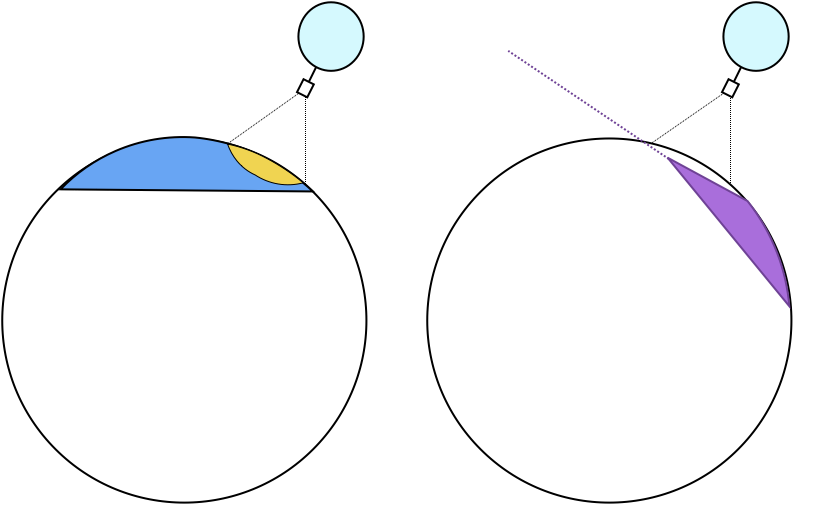
\includegraphics[width=.8\linewidth, trim = 0 6.5cm 0 0, clip]{./Figs/icemcWeightScheme.png}
  \caption{A schematic of the phase space weights used in \icemc. The
    position weight arises because only interaction positions within
    the balloon horizon are simulated (yellow over blue area).
  The direction weight arises because only favourable directions around the
  Cherenkov cone are simulated (purple angle over a unit sphere).}
  \label{fig:weights}
\end{figure}
